\section{Experimental Results}
\label{sec:experiments}

We evaluate Kimodo-Policy through single- and multi-task HumanoidArena control (Sec.~\ref{sec:exp_simulation}), SIMPLE manipulation (Sec.~\ref{sec:exp_simple}), and real-world deployment (Sec.~\ref{sec:exp_real}). Analyses cover T2M backbone quality (Sec.~\ref{sec:exp_t2m}), data and model scaling (Sec.~\ref{sec:exp_scaling}), and design ablations (Sec.~\ref{sec:exp_ablation}). Appendix~\ref{sec:experimental_setup} details the datasets, training protocols, and evaluation environments.

\subsection{Evaluation on the HumanoidArena Benchmark}
\label{sec:exp_simulation}

HumanoidArena~\cite{humanoidarena} covers seven language-conditioned tasks spanning human--object interaction (HOI) and human--scene interaction (HSI). We evaluate independent per-task fine-tuning and joint training across SONIC tasks. Appendix~\ref{sec:vis_humanoidarena} (Fig.~\ref{fig:humanoidarena}) visualizes the tasks.

\begingroup
\setlength{\intextsep}{6pt plus 1pt minus 1pt}
\textbf{Single-task results.} We fine-tune one policy per task with RTC disabled to match baselines. Kimodo-Policy uses direct task fine-tuning; Kimodo-Policy$^{*}$ initializes ControlNet and the hand head from our 419-hour VLA pretraining. Kimodo-Policy achieves the highest overall success rate (SR; 69.51\%), exceeding the strongest baseline, DP~\cite{chi2023diffusionpolicy} (60.0\%), by 9.51 percentage points. It also leads in average HSI SR (84.58\%) and ties Kimodo-Policy$^{*}$ for lowest average fall rate (AFR; 4.29\%). Kimodo-Policy$^{*}$ achieves 67.14\% overall and 84.17\% average HSI SR, leading OpenDoor (93.3\%) and VisNavi (76.7\%). VLA pretraining improves selected tasks, while direct fine-tuning yields higher overall SR.




  




\begin{table}[H]
  \setlength{\belowcaptionskip}{6pt}
  \caption{\textbf{\textit{Single-task HumanoidArena results.}} A separate policy is fine-tuned per task. For Tables~\ref{tab:arena_single_task}--\ref{tab:arena_multi_task}, values are mean $\pm$ standard deviation; $^{*}$ marks VLA-pretrained initialization, and bold/underlined entries mark best/second-best results.}
  \label{tab:arena_single_task}
  \centering
  \arrayrulecolor{hclblue}
  \begin{adjustbox}{max width=\textwidth}
  \setlength{\tabcolsep}{4.2pt}
  \renewcommand{\arraystretch}{1.08}

  \begin{tabular}{ccccc|ccccc}
  \toprule
  & &
  \multicolumn{3}{c|}{\textbf{Human--Object Interaction}} &
  \multicolumn{4}{c}{\textbf{Human--Scene Interaction}} & \\
  \cmidrule(lr){3-5}
  \cmidrule(lr){6-9}

  \multirow{-2}{*}{\textbf{Method}} &
  \multirow{-2}{*}{\textbf{AFR~($\downarrow$)}} &
  \textbf{\textsc{Football}} &
  \textbf{\textsc{DoubleDesk}} &
  \textbf{\textsc{P\&Pbox}} &
  \textbf{\textsc{OpenDoor}} &
  \textbf{\textsc{SitSofa}} &
  \textbf{\textsc{Boxing}} &
  \textbf{\textsc{VisNavi}} &
  \multirow{-2}{*}{\textbf{\textsc{Overall~($\uparrow$)}}} \\
  
  \midrule
  ACT~\cite{ACT}
  & 8.57\%
  & 16.7$\pm$6.2\%
  & 18.3$\pm$4.7\%
  & 56.7$\pm$6.2\%
  & 78.3$\pm$9.4\%
  & 73.3$\pm$8.5\%
  & 56.7$\pm$6.2\%
  & 33.3$\pm$2.4\%
  & 47.61\% \\

  DP~\cite{chi2023diffusionpolicy}
  & 8.33\%
  & \textbf{45.0$\pm$10.8\%}
  & 36.7$\pm$4.7\%
  & 75.0$\pm$4.1\%
  & 85.0$\pm$10.8\%
  & 78.3$\pm$14.3\%
  & \textbf{76.7$\pm$2.4\%}
  & 23.3$\pm$6.2\%
  & 60\% \\

  FM~\cite{FM_objective}
  & 5.71\%
  & 13.3$\pm$2.4\%
  & 38.3$\pm$4.7\%
  & 73.3$\pm$6.2\%
  & 70.0$\pm$4.1\%
  & 15.0$\pm$14.7\%
  & 70.0$\pm$8.2\%
  & 38.3$\pm$14.3\%
  & 45.46\% \\

  $\pi_{0.5}$~\cite{pi05}
  & \underline{5.24\%}
  & 10.0$\pm$4.1\%
  & \textbf{43.3$\pm$6.2\%}
  & 71.7$\pm$11.8\%
  & 66.7$\pm$6.2\%
  & 73.3$\pm$2.4\%
  & 70.0$\pm$0.0\%
  & 23.3$\pm$6.2\%
  & 51.19\% \\

  \rowcolor{hclbrown!8!white}
  \texttt{Ours}
  & \textbf{4.29\%}
  & \underline{28.3$\pm$6.2\%}
  & \underline{40.0$\pm$0.0\%}
  & \textbf{80.0$\pm$4.1\%}
  & \underline{90.0$\pm$4.1\%}
  & \textbf{100.0$\pm$0.0\%}
  & \underline{73.3$\pm$13.1\%}
  & \underline{75.0$\pm$10.8\%}
  & \textbf{69.51\%} \\


  \rowcolor{hclbrown!15!white}
  \texttt{Ours}$^{*}$
  & \textbf{4.29\%}
  & 26.7$\pm$4.7\%
  & 28.3$\pm$2.4\%
  & \underline{78.3$\pm$8.5\%}
  & \textbf{93.3$\pm$2.4\%}
  & \underline{96.7$\pm$2.4\%}
  & 70.0$\pm$8.2\%
  & \textbf{76.7$\pm$18.9\%}
  & \underline{67.14\%} \\

  \bottomrule
  \end{tabular}
  \end{adjustbox}
\end{table}


\textbf{Multi-task results.} We jointly train one policy on all seven HumanoidArena tasks and evaluate under SONIC~\cite{humanoidarena,sonic}, with RTC disabled to match baselines. Table~\ref{tab:arena_multi_task} shows Kimodo-Policy$^{*}$ reaching 72.14\% overall SR, exceeding the strongest baseline, $\pi_{0.5}$~\cite{pi05} (53.8\%), by 18.33 percentage points, with lowest AFR (4.29\%). It leads HOI (56.11\%) and HSI (84.17\%) averages, P\&Pbox (90.0\%), OpenDoor (95.0\%), SitSofa (96.7\%, tied), and VisNavi (76.7\%). Without VLA pretraining, Kimodo-Policy reaches 67.63\% overall and 51.67\% HOI SR; overall SR falls only 1.88 percentage points from single-task training. Thus, a shared policy can retain much of its single-task performance with high success and low fall rates.

\begin{table}[H]
  \setlength{\belowcaptionskip}{6pt}
  \caption{\textbf{\textit{Multi-task HumanoidArena results.}} One policy is jointly trained on all seven tasks.}
  \label{tab:arena_multi_task}
  \centering
  \arrayrulecolor{hclblue}
  \begin{adjustbox}{max width=\textwidth}
  \setlength{\tabcolsep}{4.2pt}
  \renewcommand{\arraystretch}{1.08}

  \begin{tabular}{ccccc|ccccc}
  \toprule
  & &
  \multicolumn{3}{c|}{\textbf{Human--Object Interaction}} &
  \multicolumn{4}{c}{\textbf{Human--Scene Interaction}} & \\
  \cmidrule(lr){3-5}
  \cmidrule(lr){6-9}

  \multirow{-2}{*}{\textbf{Method}} &
  \multirow{-2}{*}{\textbf{AFR~($\downarrow$)}} &
  \textbf{\textsc{Football}} &
  \textbf{\textsc{DoubleDesk}} &
  \textbf{\textsc{P\&Pbox}} &
  \textbf{\textsc{OpenDoor}} &
  \textbf{\textsc{SitSofa}} &
  \textbf{\textsc{Boxing}} &
  \textbf{\textsc{VisNavi}} &
  \multirow{-2}{*}{\textbf{\textsc{Overall~($\uparrow$)}}} \\
  \midrule

  ACT~\cite{ACT}
  & 7.4\%
  & 20.0$\pm$4.1\%
  & 30.0$\pm$4.1\%
  & 60.0$\pm$12.2\%
  & 58.3$\pm$2.4\%
  & 21.7$\pm$2.4\%
  & 58.3$\pm$10.3\%
  & 28.3$\pm$4.7\%
  & 39.5\% \\

  DP~\cite{chi2023diffusionpolicy}
  & 7.1\%
  & \textbf{53.3$\pm$6.2\%}
  & 35.0$\pm$10.8\%
  & 0.0$\pm$0.0\%
  & 83.3$\pm$6.2\%
  & \underline{83.3$\pm$4.7\%}
  & 21.7$\pm$30.6\%
  & 50.0$\pm$14.7\%
  & 46.7\% \\

  FM~\cite{FM_objective}
  & 7.1\%
  & 21.7$\pm$8.5\%
  & 20.0$\pm$7.1\%
  & 0.0$\pm$0.0\%
  & 76.7$\pm$2.4\%
  & 48.3$\pm$6.2\%
  & 18.3$\pm$25.9\%
  & 38.3$\pm$6.2\%
  & 31.9\% \\

  $\pi_{0.5}$~\cite{pi05}
  & 6.4\%
  & 10.0$\pm$7.1\%
  & 30.0$\pm$7.1\%
  & 75.0$\pm$4.1\%
  & 85.0$\pm$4.1\%
  & 70.0$\pm$14.7\%
  & \textbf{71.7$\pm$12.5\%}
  & 35.0$\pm$4.1\%
  & 53.8\% \\

  \rowcolor{hclbrown!8!white}
  \texttt{Ours}
  & \underline{5.0\%}
  & 35.0$\pm$7.1\%
  & \textbf{40.0$\pm$0.0\%}
  & \underline{80.0$\pm$4.1\%}
  & \underline{93.3$\pm$6.2\%}
  & \textbf{96.7$\pm$4.7\%}
  & 66.7$\pm$4.7\%
  & \underline{61.7$\pm$6.2\%}
  & \underline{67.6\%} \\


  \rowcolor{hclbrown!15!white}
  \texttt{Ours}$^{*}$
  & \textbf{4.3\%}
  & \underline{40.0$\pm$4.1\%}
  & \underline{38.3$\pm$2.4\%}
  & \textbf{90.0$\pm$4.1\%}
  & \textbf{95.0$\pm$4.1\%}
  & \textbf{96.7$\pm$4.7\%}
  & \underline{68.3$\pm$10.3\%}
  & \textbf{76.7$\pm$8.5\%}
  & \textbf{72.1\%} \\



  \bottomrule
  \end{tabular}
  \end{adjustbox}
\end{table}


\textbf{Attention map analysis.} Figure~\ref{fig:attention} shows Kimodo-Policy focusing on the ball in Football, box in P\&P Box, and punching bag in Boxing, alongside relevant scene elements for door opening, sitting, and navigation. $\pi_{0.5}$ responds less locally, while Diffusion Policy activates broader scene regions. This task-dependent focus suggests alignment with instruction semantics and use of task-relevant cues for shared multi-task action selection.

\begin{figure}[H]
  \centering
  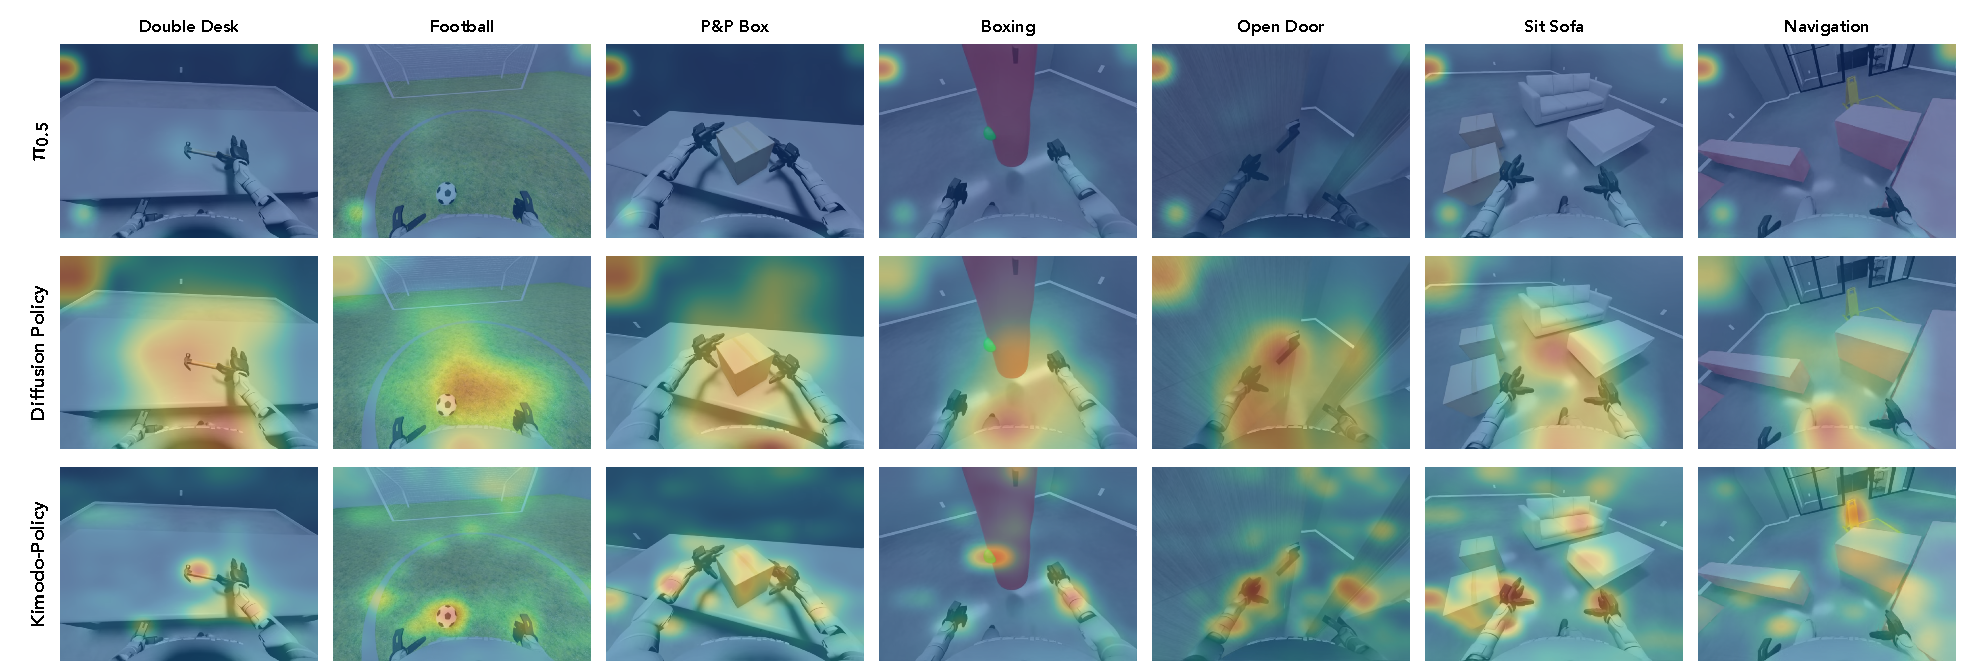
\includegraphics[width=\textwidth]{image/attention.pdf}
  \caption{\textbf{Task-Conditioned Visual Attention.} Columns show seven HumanoidArena tasks; rows (top to bottom) show $\pi_{0.5}$, Diffusion Policy, and Kimodo-Policy. Kimodo-Policy shifts attention toward task-relevant objects and interaction regions.}
  \label{fig:attention}
\end{figure}
\endgroup

\begingroup
\setlength{\intextsep}{6pt plus 1pt minus 1pt}
\subsection{Evaluation on the Simple Benchmark}
\label{sec:exp_simple}
We further evaluate Kimodo-Policy on the SIMPLE benchmark~\cite{simple}, using the L0--L2 protocol with progressively stronger visual, lighting, and target-pose randomization~\cite{simple}. We fine-tune an independent policy for each of the eight benchmark tasks and report the results in Table~\ref{table:simple_main_results}. This protocol isolates skill acquisition while testing robustness under increasing distribution shifts. See Appendix~\ref{sec:vis_simple} (Fig.~\ref{fig:simple_tasks}) for task visualizations.



\textbf{Single-task results.} Table~\ref{table:simple_main_results} evaluates VLA-pretrained Kimodo-Policy (\texttt{Ours}$^{*}$) on eight SIMPLE tasks, aggregating L0--L2 success rates with RTC disabled to match the baselines. It achieves best or joint-best results on six tasks: Handover (83\% vs. 80\% for the strongest baseline), Mobile P\&P (70\% vs. 60\%), OpenOven (57\% vs. 53\%), OpenFaucet (53\% vs. 33\%), CloseDoor and Push Office Chair (both 100\%, tied with $\Psi_0$). It ranks second on XMoveBendPick (80\% vs. 93\% for $\Psi_0$) and OpenTrashCan (63\% vs. 83\%). These results show that the motion-prior-based, visually grounded root--body--hand policy supports handover, mobile manipulation, articulated-object interaction, and pushing under visual, lighting, and target-pose variation.

\begin{table}[H]
  \setlength{\belowcaptionskip}{6pt}
  \caption{\textbf{\textit{Single-Task Results on SIMPLE.}} L0--L2 progressively increase visual and lighting variation and target-pose randomization. Entries report L0/L1/L2 success counts and aggregate success rates (parentheses); bold/underlined values mark the best/second-best aggregate rates.}
  \label{table:simple_main_results}
  \centering
  \arrayrulecolor{hclblue}
  \setlength{\tabcolsep}{0pt}
  \renewcommand{\arraystretch}{1.08}
  \fontsize{6.2}{7}\selectfont
  \newcommand{\taskheader}[1]{{\fontsize{5.55}{6.2}\selectfont\textbf{\textsc{\hspace{2.2pt}#1\hspace{2.2pt}}}}}
  \newcommand{\resultentry}[2]{{\fontsize{5.2}{6}\selectfont\hspace{2.2pt}#1\;(#2)\hspace{2.2pt}}}
  \newcommand{\bestentry}[2]{{\fontsize{5.2}{6}\selectfont\textbf{\hspace{2.2pt}#1\;(#2)\hspace{2.2pt}}}}
  \newcommand{\secondentry}[2]{{\fontsize{5.2}{6}\selectfont\hspace{2.2pt}\underline{#1\;(#2)}\hspace{2.2pt}}}

  \begin{adjustbox}{width=\textwidth}
  \begin{tabular}{@{}c*{8}{c}@{}}
    \toprule
    {\fontsize{5.55}{6.2}\selectfont\textbf{Method}}
    & \taskheader{Handover}
    & \taskheader{Mobile P\&P}
    & \taskheader{XMoveBendPick}
    & \taskheader{CloseDoor}
    & \taskheader{OpenOven}
    & \taskheader{OpenFaucet}
    & \taskheader{Push Office Chair}
    & \taskheader{OpenTrashCan} \\
    \midrule

    $\Psi_0$~\cite{psi0}
    & \secondentry{7/7/10}{80\%}
    & \secondentry{7/5/6}{60\%}
    & \bestentry{10/9/9}{93\%}
    & \bestentry{10/10/10}{100\%}
    & \secondentry{7/5/4}{53\%}
    & \secondentry{3/3/4}{33\%}
    & \bestentry{10/10/10}{100\%}
    & \bestentry{7/9/9}{83\%} \\

    \rowcolor{hclbrown!15!white}
    \texttt{Ours}$^{*}$
    & \bestentry{9/8/8}{83\%}
    & \bestentry{9/8/4}{70.0\%}
    & \secondentry{10/7/7}{80\%}
    & \bestentry{10/10/10}{100\%}
    & \bestentry{8/4/5}{57\%}
    & \bestentry{5/6/5}{53\%}
    & \bestentry{10/10/10}{100\%}
    & \secondentry{9/4/6}{63\%} \\

    \bottomrule
  \end{tabular}
  \end{adjustbox}
\end{table}


\subsection{Evaluation on the Real-World Humanoid Robot}
\label{sec:exp_real}
We test a physical humanoid on eight language-conditioned loco-manipulation tasks under unconstrained sensing and execution, covering locomotion, balance, single- and dual-arm coordination, and contact-rich manipulation. Each task has ten trials scored by successful completions; Appendix~\ref{sec:vis_real_world} (Fig.~\ref{fig:real_world}) provides visualizations.

\textbf{Real-world results.} Scratch-trained Kimodo-Policy averages 45\% success, above GR00T N1.6~\cite{grootn1} (31\%) and $\Psi_0$~\cite{psi0} (35\%; Fig.~\ref{fig:real_world_success_rates}). VLA pretraining raises this to 60\% (+15 points), improving seven tasks and matching Cart Pushing (60\%). Its strongest results are Punching Bag (90\%), Cushion Sitting (80\%), and Dual-Arm PNP (70\%).

\begin{figure}[H]
  \centering
  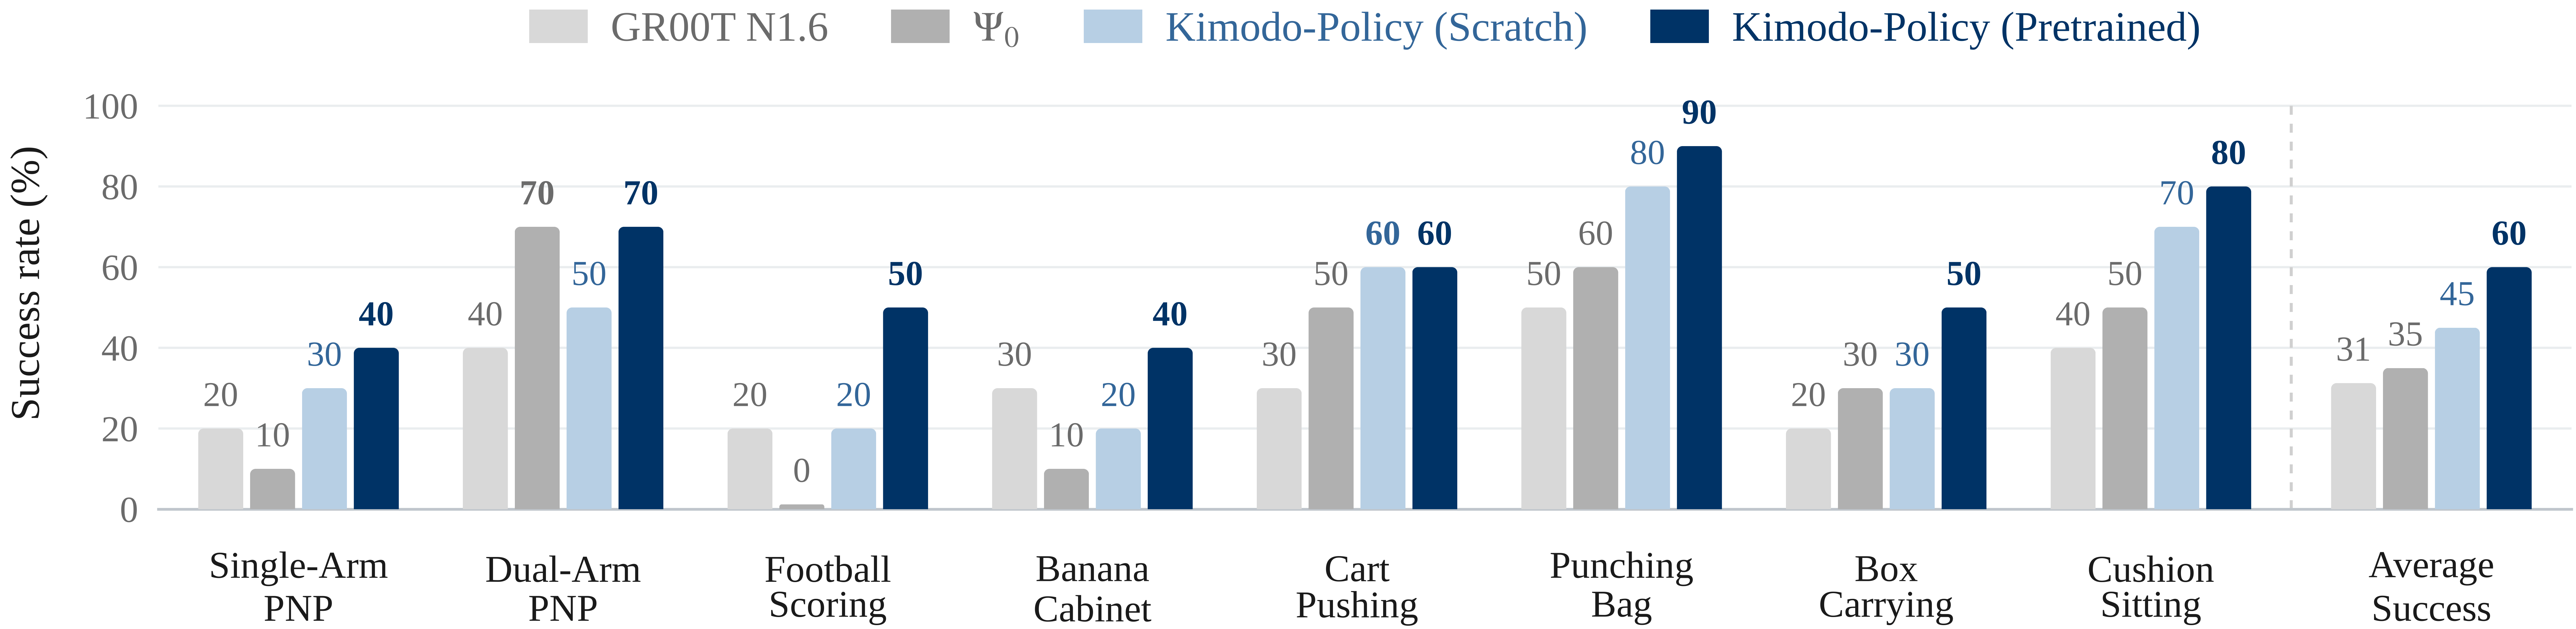
\includegraphics[width=\textwidth]{image/real_world_success_rates.png}
  \caption{\textbf{Real-World Success Rates.} GR00T N1.6, $\Psi_0$, and Kimodo-Policy with/without VLA pretraining are compared on eight tasks; the rightmost group reports mean success.}
  \label{fig:real_world_success_rates}
\end{figure}

\subsection{Does Better T2M Improve VLA Performance?}
\label{sec:exp_t2m}
To test motion-prior quality, we compare Kimodo-G1-SEED-v1 and RP-v1 T2M backbones~\cite{kimodo} under identical policy architectures, adaptation procedures, and HumanoidArena protocols. Both have 282M parameters and 90\%/10\% train/test splits; SEED-v1 uses 288\,h of BONES-SEED data and RP-v1 uses 700\,h of Rigplay~\cite{kimodo}.
\begin{table}[H]
  \setlength{\belowcaptionskip}{6pt}
  \caption{
    \textbf{\textit{Effect of the T2M backbone on Kimodo-Policy.}} We compare two same-size Kimodo-G1 backbones using the same adaptation protocol. Data scales include the training and test splits; results are mean $\pm$ standard deviation over three seeds.}
  \label{tab:t2m_dependency}
  \centering
  \arrayrulecolor{hclblue}
  \begin{adjustbox}{max width=\textwidth}
  \setlength{\tabcolsep}{3.8pt}
  \renewcommand{\arraystretch}{1.08}

  \begin{tabular}{cccccc|ccccc}
  \toprule
  \multirow{2}{*}{\textbf{Base Model}} &
  \multirow{2}{*}{\textbf{Model Size}} &
  \multirow{2}{*}{\textbf{Data Scale}} &
  \multicolumn{3}{c|}{\textbf{Human--Object Interaction}} &
  \multicolumn{4}{c}{\textbf{Human--Scene Interaction}} &
  \multirow{2}{*}{\textbf{Overall~($\uparrow$)}} \\
  \cmidrule(lr){4-6}
  \cmidrule(lr){7-10}

  & & &
  \textbf{\textsc{Football}} &
  \textbf{\textsc{DoubleDesk}} &
  \textbf{\textsc{P\&Pbox}} &
  \textbf{\textsc{OpenDoor}} &
  \textbf{\textsc{SitSofa}} &
  \textbf{\textsc{Boxing}} &
  \textbf{\textsc{VisNavi}} \\
  \midrule

  \texttt{Kimodo-G1-SEED-v1}
  & 282\,M
  & 288\,h
  & \textbf{50.00$\pm$16.33\%}
  & \underline{33.33$\pm$15.46\%}
  & \underline{75.00$\pm$10.80\%}
  & \underline{60.00$\pm$4.08\%}
  & \underline{90.00$\pm$4.08\%}
  & \textbf{71.67$\pm$8.50\%}
  & \textbf{70.00$\pm$18.71\%}
  & \underline{64.29\%} \\

  \rowcolor{hclbrown!8!white}
  \texttt{Kimodo-G1-RP-v1}
  & 282\,M
  & 700\,h
  & \underline{35.0$\pm$7.1\%}
  & \textbf{40.0$\pm$0.0\%}
  & \textbf{80.0$\pm$4.1\%}
  & \textbf{93.3$\pm$6.2\%}
  & \textbf{96.7$\pm$4.7\%}
  & \underline{66.7$\pm$4.7\%}
  & \underline{61.7$\pm$6.2\%}
  & \textbf{67.63\%} \\

  \bottomrule
  \end{tabular}
  \end{adjustbox}
\end{table}

\textbf{T2M transfer results.} RP-v1 improves overall SR over SEED-v1 from 64.29\% to 67.63\% (+3.34 points; Table~\ref{tab:t2m_dependency}), with gains on DoubleDesk ($33.33\%\to40.0\%$), P\&Pbox ($75.0\%\to80.0\%$), OpenDoor ($60.0\%\to93.3\%$), and SitSofa ($90.0\%\to96.7\%$), but declines on Football ($50.0\%\to35.0\%$), Boxing ($71.67\%\to66.7\%$), and VisNavi ($70.0\%\to61.7\%$). Gains concentrate in human--scene interaction, with task-dependent trade-offs.

\subsection{Does Performance Scale with Data and Model Size?}
\label{sec:exp_scaling}
We vary VLA policy-pretraining data duration with the architecture, SonicX7 adaptation, and evaluation fixed, then vary active policy parameters with the pretrained T2M backbone, downstream data, optimization, and evaluation fixed. RTC is disabled throughout to match the benchmark protocol.

\begin{figure}[H]
  \centering
  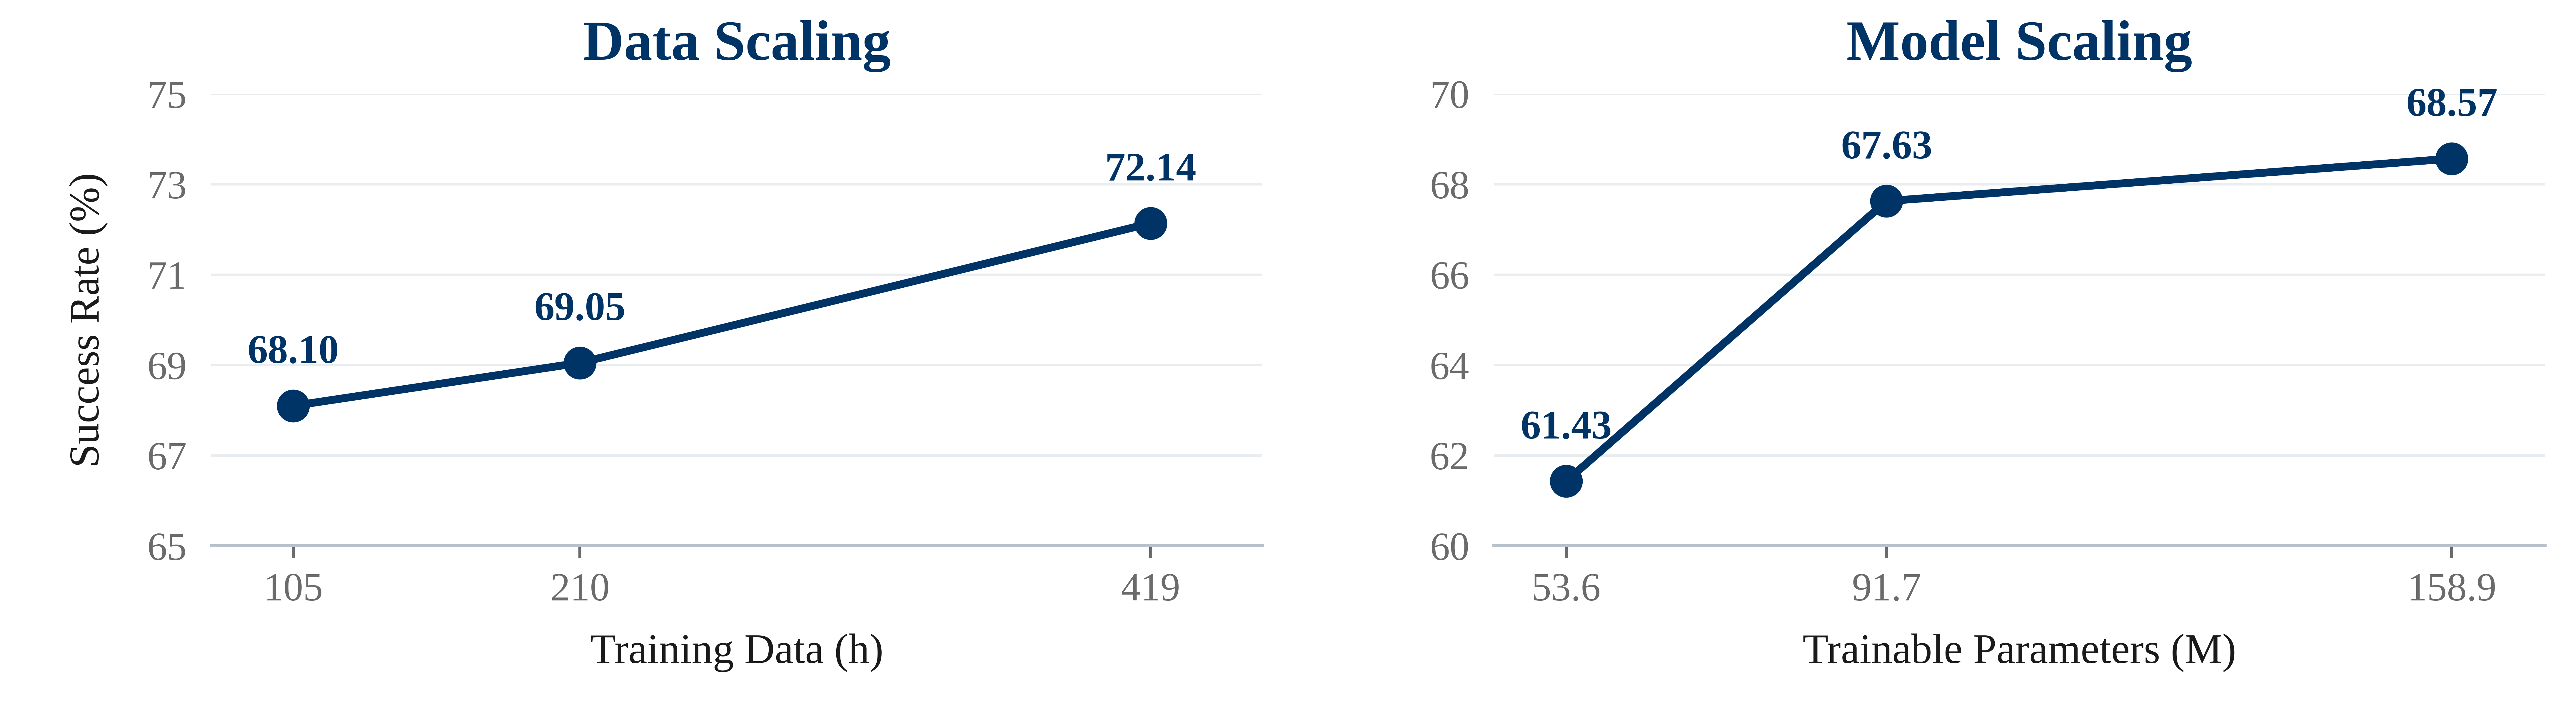
\includegraphics[width=\textwidth]{image/scaling_analysis.png}
  \caption{Scaling behavior of Kimodo-Policy. Left: overall success rate as a function of VLA policy-pretraining data duration. Right: overall success rate as a function of active policy parameters.}
  \label{fig:scaling_analysis}
\end{figure}

\textbf{Data scaling results.} Overall success rises from 68.10\% with 105\,h to 69.05\% with 210\,h and 72.14\% with 419\,h of VLA pretraining data, a 4.04-point gain (Fig.~\ref{fig:scaling_analysis}).

\textbf{Model scaling results.} Increasing active policy parameters from 53.6M to 91.7M and 158.9M raises overall success from 61.43\% to 67.63\% and 68.57\%, respectively, a 7.14-point gain that supports scaling policy capacity.

\begingroup
% Use the official ICLR subsection formatting.
\subsection{Ablation Study}
\label{sec:exp_ablation}
\color{black}
All ablations train on mixed HumanoidArena tasks in SONIC X7 and evaluate on DoubleDesk, Football, and P\&Pbox. Figure~\ref{fig:training_loss_comparison} reports training loss and mean success across these tasks.
\begin{figure}[H]
  \centering
  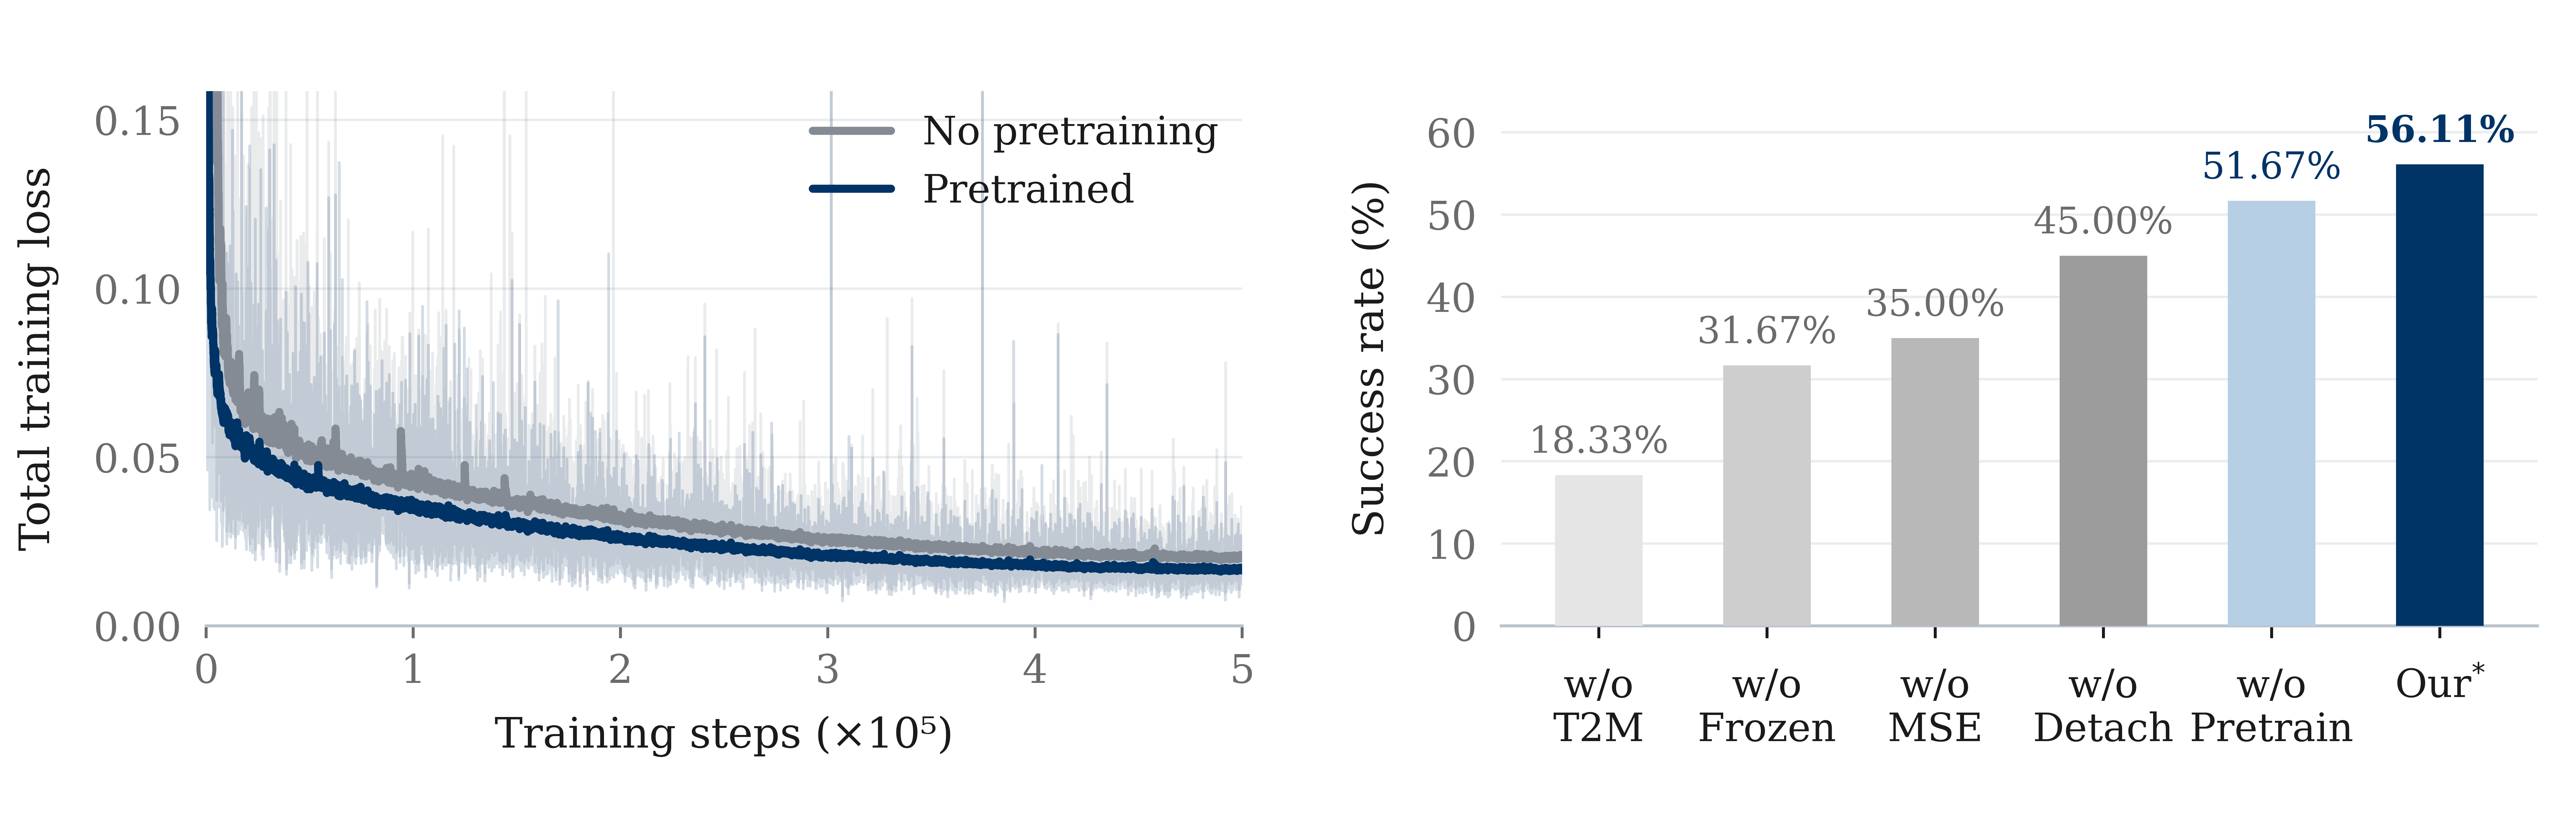
\includegraphics[width=\textwidth]{image/training_loss_comparison.png}
  \caption{\textbf{Training Dynamics and Ablations.} Left: training loss with/without VLA pretraining. Right: mean success on DoubleDesk, Football, and P\&Pbox. Gray: component and training-design ablations; light/dark blue: without/with VLA pretraining.}
  \label{fig:training_loss_comparison}
\end{figure}



\textbf{Results Analysis.} Without VLA pretraining, Kimodo-Policy achieves 51.67\% mean success; removing the T2M backbone, unfreezing it, replacing MSE with Kimodo's original motion objective, or removing root--body gradient detachment yields 18.33\%, 31.67\%, 35.00\%, or 45.00\%, respectively. These results support a frozen motion prior, MSE supervision, and gradient separation. VLA pretraining raises success from 51.67\% to 56.11\%, with generally lower and less variable training loss. Both variants retain the T2M backbone, indicating complementary benefits.

\endgroup
\endgroup
